\documentclass[11pt]{article}

% ---------- Packages ----------
\usepackage[a4paper,margin=1in]{geometry}
\usepackage{microtype}
\usepackage{amsmath,amssymb,amsthm}
\usepackage{mathtools}
\usepackage{booktabs,longtable,tabularx,array}
\usepackage{enumitem}
\usepackage{hyperref}
\usepackage{xcolor}
\usepackage{graphicx}
\usepackage{tikz}
\usetikzlibrary{arrows.meta,positioning,calc,fit,shapes.geometric}
\usepackage{algorithm}
\usepackage{algpseudocode}
\usepackage{caption}
\usepackage{subcaption}
\usepackage{adjustbox}
\usepackage{siunitx}
\usepackage{float}

% ---------- Hyperref ----------
\hypersetup{
  colorlinks=true,
  linkcolor=blue,
  citecolor=blue,
  urlcolor=blue,
  pdftitle={Component 2: Technical Documentation},
  pdfauthor={Fact-or-Fiction Project},
}

% ---------- List spacing ----------
\setlist[itemize]{leftmargin=*,topsep=2pt,itemsep=2pt}
\setlist[enumerate]{leftmargin=*,topsep=2pt,itemsep=2pt}

% ---------- Notation helpers ----------
\newcommand{\sigmoid}{\operatorname{sigmoid}}
\newcommand{\softmax}{\operatorname{softmax}}
\newcommand{\PPR}{\operatorname{PPR}}
\newcommand{\Rel}{\operatorname{Rel}}
\newcommand{\Pol}{\operatorname{Pol}}
\newcommand{\Conn}{\operatorname{Conn}}
\newcommand{\AURC}{\operatorname{AURC}}

\title{\textbf{Component 2 Documentation (Academic Version)}\\
PV-Aware Graph Reasoning, Bridge Rescue, Recovery, and Reliability Metrics}
\author{Fact-or-Fiction Project}
\date{Code-aligned revision date: February 10, 2026}

\begin{document}
\maketitle

\begin{abstract}
This document is a code-aligned technical specification for \texttt{src/component2/} in the Fact-or-Fiction repository.
It is written to support two goals simultaneously: (i) concept-level understanding for explanation and teaching, and (ii) exact implementation-level traceability for development and review.
Every major equation, default value, trigger condition, input schema, and output schema is mapped to the current code and milestone runners (M1, M2, M3).
The document is split into multiple \LaTeX{} files for maintainability.
\end{abstract}

\tableofcontents
\newpage

\section{Scope, Objectives, and Pipeline Placement}
\label{sec:scope}

\subsection{What Component 2 is responsible for}
Component 2 is the graph reasoning stage that consumes Component 1 outputs and produces a robust claim-level decision.
The implementation target is FactKG-style KG fact verification \cite{kim2023factkg}, within the Fact-or-Fiction pipeline \cite{opsahl2024factorfiction}.
It is explicitly designed to preserve contradictory signal, reduce neutral/noisy propagation, and recover structurally important edges when evidence is insufficient.

\textbf{Primary objectives:}
\begin{itemize}
\item Use PV scores from Component 1 as soft control signals during graph reasoning.
\item Keep support and refute evidence streams separate until graph-level fusion.
\item Detect bridge-like evidence in Suspended pool $S$ with diffusion instead of costly path enumeration.
\item Trigger one-step recovery only when insufficiency and predicted connectivity gain are both present.
\item Expose reliability outputs: abstain scores, risk-coverage metrics, and rationale faithfulness checks.
\end{itemize}

\subsection{Position in the full pipeline}
\begin{figure}[H]
\centering
\begin{adjustbox}{max width=\textwidth}
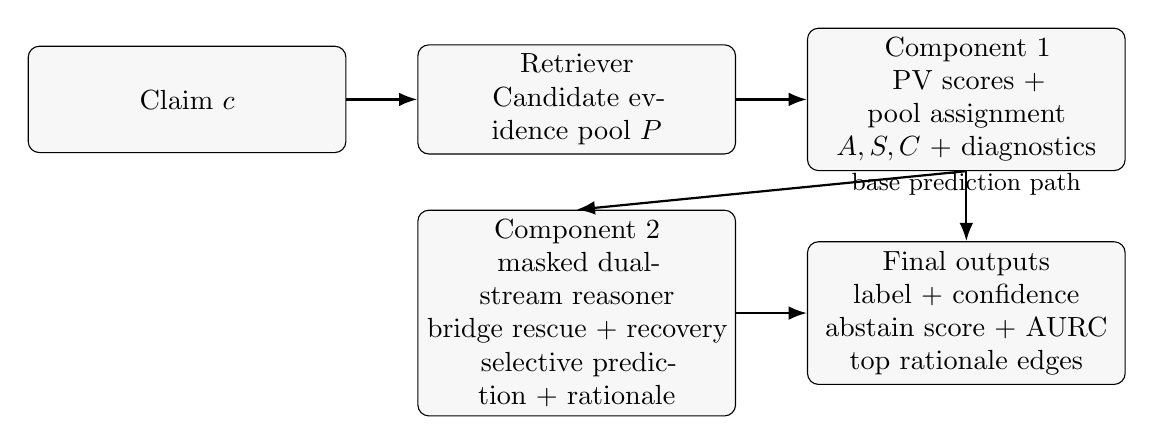
\begin{tikzpicture}[
  node distance=7mm and 9mm,
  block/.style={draw,rounded corners,align=center,text width=3.8cm,minimum height=1.35cm,fill=gray!6},
  arrow/.style={-Latex,thick}
]
\node[block] (claim) {Claim $c$};
\node[block, right=of claim] (retriever) {Retriever\\Candidate evidence pool $P$};
\node[block, right=of retriever] (comp1) {Component 1\\PV scores + pool assignment\\$A, S, C$ + diagnostics};
\node[block, below=of retriever] (comp2) {Component 2\\masked dual-stream reasoner\\bridge rescue + recovery\\selective prediction + rationale};
\node[block, right=of comp2] (output) {Final outputs\\label + confidence\\abstain score + AURC\\top rationale edges};

\draw[arrow] (claim) -- (retriever);
\draw[arrow] (retriever) -- (comp1);
\draw[arrow] (comp1.south) -- (comp2.north);
\draw[arrow] (comp2) -- (output);
\draw[arrow] (comp1) -- node[above,font=\small]{base prediction path} (output);
\end{tikzpicture}
\end{adjustbox}
\caption{Page-fitted system view with Component 2 in context.}
\label{fig:pipeline-overview}
\end{figure}

\subsection{Milestone structure in code}
The code is organized as progressive milestones, each with a dedicated runner:
\begin{itemize}
\item \textbf{M1:} \texttt{src/component2/run\_m1.py} (core reasoner + salience logging).
\item \textbf{M2:} \texttt{src/component2/run\_m2.py} (bridge rescue and policy-aware recovery).
\item \textbf{M3:} \texttt{src/component2/run\_m3.py} (selective prediction and rationale faithfulness checks).
\end{itemize}

\subsection{Core symbols used throughout}
\begin{table}[H]
\centering
\begin{tabular}{@{}p{0.2\linewidth}p{0.72\linewidth}@{}}
\toprule
Symbol & Meaning \\
\midrule
$c$ & Claim text instance. \\
$e$ & Evidence triple $e=(s,r,o)$ with PV scores. \\
$A,S,C$ & Active, Suspended, Counter pools from Component 1. \\
$\Rel(e)$ & Decision relevance mass: $p_{\text{ent}}(e)+p_{\text{con}}(e)$. \\
$\Pol(e)$ & Polarity: $p_{\text{ent}}(e)-p_{\text{con}}(e)$. \\
$\Conn(\cdot)$ & Anchor-pair connectivity fraction on Active graph. \\
$\PPR$ & Personalized PageRank diffusion used for bridge scoring. \\
\bottomrule
\end{tabular}
\caption{Minimal notation used across all Component 2 modules.}
\label{tab:core-notation}
\end{table}

\section{Data Contract: Inputs, Validation Rules, and Outputs}
\label{sec:contract}

\subsection{Primary claim input format (triples JSONL mode)}
The standard input to Component 2 is a JSONL file where each row is normalized to \texttt{ClaimRecord} in \texttt{src/component2/types.py}.

\begin{table}[H]
\centering
\begin{tabular}{@{}p{0.26\linewidth}p{0.18\linewidth}p{0.50\linewidth}@{}}
\toprule
Field & Type & Semantics \\
\midrule
\texttt{claim\_id} & string & Required unique claim identifier. Empty values are rejected. \\
\texttt{claim\_text} & string & Claim text. Fallback key accepted: \texttt{Sentence}. \\
\texttt{label} & string/null & Optional. Mapped to class index: SUPPORT$\to0$, REFUTE$\to1$. \\
\texttt{entity\_set} & list/string & Claim seed entities used for anchor selection. Fallback key: \texttt{Entity\_set}. \\
\texttt{triples} & list & Required per-claim evidence list. Each item must be a valid evidence triple. \\
\texttt{sufficiency} & object & Optional diagnostic map; \texttt{esi\_geom} is consumed by recovery/abstention. \\
\bottomrule
\end{tabular}
\caption{Claim-level schema accepted by \texttt{claim\_from\_dict}.}
\label{tab:claim-schema}
\end{table}

\subsection{Per-evidence schema and derived values}
Each evidence row is normalized to \texttt{EvidenceTriple}.

\begin{table}[H]
\centering
\begin{tabular}{@{}p{0.26\linewidth}p{0.18\linewidth}p{0.50\linewidth}@{}}
\toprule
Field & Type & Semantics \\
\midrule
\texttt{evidence\_id} & string & Required unique id within claim. Duplicates are rejected. \\
\texttt{raw\_triple} & 3-tuple/list & Required $(subject, relation, object)$ triple. \\
\texttt{pool} & string & One of \texttt{A}, \texttt{S}, \texttt{C}. \\
\texttt{p\_ent}, \texttt{p\_con}, \texttt{p\_neu} & float & Required probabilities in $[0,1]$ and finite. \\
\texttt{probs} (alternative) & object & Accepted as \{entail, contra, neutral\} or \{p\_ent, p\_con, p\_neu\}. \\
\bottomrule
\end{tabular}
\caption{Evidence-level schema and accepted key variants.}
\label{tab:evidence-schema}
\end{table}

Derived values used by downstream modules:
\begin{align}
\Rel(e) &= p_{\text{ent}}(e) + p_{\text{con}}(e), \\
\Pol(e) &= p_{\text{ent}}(e) - p_{\text{con}}(e).
\end{align}

\subsection{Validation behavior (strictness of parser)}
\texttt{src/component2/types.py} enforces the following:
\begin{itemize}
\item Non-finite probabilities and values outside $[0,1]$ raise errors.
\item Unknown pool labels raise errors.
\item Missing or malformed triples (not length 3) raise errors.
\item Empty claim batches are rejected by \texttt{ensure\_non\_empty\_claims}.
\end{itemize}

\subsection{Component 1 compatibility mode (claims + pairs logs)}
\label{subsec:component1-compat}
\texttt{run\_m3.py} supports an alternate loader for Component 1 logs:
\begin{itemize}
\item Claims file: typically \texttt{logs/component1/train/claims.jsonl}.
\item Companion pairs file: same directory, \texttt{pairs.jsonl}, required.
\item Triple reconstruction is done by grouping pair rows by \texttt{claim\_id}.
\end{itemize}

Required pair-row elements:
\begin{itemize}
\item \texttt{claim\_id}, \texttt{evidence\_id}, \texttt{raw\_triple}, \texttt{pool} (or \texttt{evidence\_assignment}), \texttt{probs}.
\item Pool aliases accepted: \texttt{A/ACTIVE}, \texttt{S/SUSPENDED}, \texttt{C/CANDIDATE}, and ids \texttt{0/1/2}.
\item Missing pool labels or partial Suspended logging raises explicit errors because recovery needs full $S$ visibility.
\end{itemize}

\subsection{Output artifacts and path pattern}
All milestones write outputs under:
\[
\texttt{<output\_root>/<milestone>/<YYYYMMDD\_HHMMSS\_microseconds>/}
\]
using \texttt{make\_run\_dir(...)} in \texttt{src/component2/io\_utils.py}.

Each run writes:
\begin{itemize}
\item \texttt{run\_config.json}
\item \texttt{summary.json}
\item \texttt{predictions.jsonl}
\end{itemize}
M3 additionally writes \texttt{risk\_coverage.json}.

\subsection{M1 output schema (\texttt{run\_m1.py})}
\begin{table}[H]
\centering
\begin{tabular}{@{}p{0.30\linewidth}p{0.62\linewidth}@{}}
\toprule
Field & Meaning \\
\midrule
\texttt{prediction} & Binary label from argmax over \texttt{probs}. \\
\texttt{prob\_supported}, \texttt{prob\_refuted} & Final class probabilities. \\
\texttt{anchors} & Selected anchors used to build graph. \\
\texttt{top\_salience} & Top-3 edges by internal salience score. \\
\bottomrule
\end{tabular}
\caption{Per-claim prediction fields in M1.}
\end{table}

\subsection{M2 output schema (\texttt{run\_m2.py})}
In addition to M1-like prediction fields, M2 logs:
\begin{itemize}
\item Recovery metrics: \texttt{rpi\_rel\_at\_k}, \texttt{rpi\_bridge\_at\_k}, \texttt{delta\_conn\_bridge\_at\_k}, \texttt{should\_recover}.
\item Selected edge ids: \texttt{selected\_rel\_ids}, \texttt{selected\_bridge\_ids}, \texttt{moved\_evidence\_ids}.
\item Bridge diagnostics over Suspended edges: \texttt{bridge\_scores\_s} with uncapped and capped scores.
\item PPR diagnostics: convergence flag, iterations, residual, anchor connectivity counters.
\end{itemize}

\subsection{M3 output schema (\texttt{run\_m3.py})}
M3 extends M2 with reliability and interpretability fields:
\begin{itemize}
\item \texttt{abstain\_score} and optional correctness indicator \texttt{is\_correct}.
\item \texttt{top\_rationale\_edges}: top-$N$ ranked by attention$\times$PV relevance.
\item \texttt{faithfulness\_loo}: leave-one-out confidence-drop report (subset of claims).
\item \texttt{salience\_results}: grouped top-$k$ removal faithfulness report.
\item \texttt{risk\_coverage.json}: full risk-coverage points and \AURC.
\end{itemize}


\section{Graph Construction and Anchor Selection}
\label{sec:graph-anchors}

\subsection{Graph object built by \texttt{GraphBuilder}}
Component 2 reasoning operates on \texttt{EvidenceGraph} with fields:
\begin{itemize}
\item \texttt{nodes}: entity strings.
\item \texttt{node\_to\_idx}: mapping from entity to node index.
\item \texttt{edges}: list of typed graph edges with PV features.
\item \texttt{anchors}: selected anchor entities.
\item \texttt{anchor\_indices}: anchor node indices that exist in graph.
\end{itemize}

\subsection{Pool-dependent graph views}
Two graph views are used in milestone runners:
\begin{itemize}
\item Active reasoning graph: \texttt{include\_pools=("A","C")}.
\item Full bridge graph: \texttt{include\_pools=("A","S","C")}.
\end{itemize}
This split ensures the base reasoner does not directly consume Suspended edges, while bridge scoring can still inspect them.

\subsection{Edge feature set}
For each edge $e$, \texttt{GraphEdge} stores:
\[
\{\texttt{relation\_id},\texttt{pool\_id},p_{\text{ent}},p_{\text{con}},p_{\text{neu}},\Rel(e),\Pol(e)\}.
\]

Relation ids come from a mutable per-run vocabulary:
\[
\texttt{relation\_to\_id}: r \mapsto 0,1,2,\dots
\]
allocated on first appearance.

\subsection{Anchor selection policy in \texttt{AnchorSelector}}
\label{subsec:anchor-policy}
Anchor selection now receives seed entities from a source-priority adapter:
\[
\texttt{provided} \rightarrow \texttt{pickle} \rightarrow \texttt{heuristic}
\]
where \texttt{pickle} means FactKG \texttt{Entity\_set} injection from
\texttt{data/factkg/factkg\_\{train|dev|test\}.pickle} when upstream records omit \texttt{entity\_set}.
The adapter lazy-loads these mappings once per run. If configured pickle paths are missing/invalid,
or no mappings can be extracted, code emits a \texttt{RuntimeWarning} and continues with
\texttt{heuristic} fallback so data-path issues are visible without breaking execution.

Given that seed input, anchor selection follows a robust fallback hierarchy and enforces practical connectivity diagnostics:
\begin{enumerate}
\item Match seed entities (from \texttt{entity\_set}) to graph entities using normalized forms.
\item If fewer than required anchors are found, use claim-text substring matches.
\item If still insufficient, add degree-based fallback entities.
\end{enumerate}

Important implementation guards:
\begin{itemize}
\item Blank entities are discarded.
\item If the graph has at least two entities, selector attempts to return at least two anchors (bounded by \texttt{anchor\_max\_k}).
\item Degree fallback uses deterministic tie-break by first appearance in graph entities.
\end{itemize}

\begin{algorithm}[H]
\caption{Anchor Selection (code-aligned)}
\begin{algorithmic}[1]
\Require claim text $c$, triples $T$, seed entities $E_{seed}$, max anchors $K$
\State $V \leftarrow$ unique valid graph entities from $T$
\If{$|V|=0$} \State return $[\ ]$ \EndIf
\State $K_{min} \leftarrow \min(2, |V|, K)$
\State $A \leftarrow$ seed matches between $E_{seed}$ and $V$
\If{$|A| \ge K_{min}$} \State return first $K$ anchors \EndIf
\State extend $A$ with text-match entities ($\text{normalize}(v) \subseteq \text{normalize}(c)$)
\If{$|A| \ge K_{min}$} \State return first $K$ anchors \EndIf
\State extend $A$ with top-degree entities in $V$ (deterministic ties)
\State return first $K$ anchors
\end{algorithmic}
\label{alg:anchor-selection}
\end{algorithm}

\subsection{Connectivity semantics used downstream}
Recovery and bridge diagnostics use undirected connectivity over Active edges.
For anchor pair $(a_i,a_j)$:
\begin{itemize}
\item if either anchor is missing from Active nodes, pair is treated as disconnected,
\item otherwise BFS/graph traversal is used to test connectivity.
\end{itemize}
The pairwise connectivity score is:
\[
\Conn(A)=\frac{\#\text{connected anchor pairs}}{\#\text{anchor pairs}}.
\]
When fewer than two unique anchors exist, implementation returns $1.0$ (degenerate no-pair case).

\section{Reasoner Mechanics: Masked Dual-Stream Hybrid GAT}
\label{sec:reasoner}

\subsection{Implemented model}
The active reasoner class is
\texttt{HybridMaskedDualStreamReasoner} in \texttt{src/component2/reasoner.py}.
It is a deterministic NumPy implementation that combines:
\begin{itemize}
\item relation-conditioned attention,
\item separate support/refute message streams,
\item fixed PV-based masking,
\item hybrid graph pooling (mean + max + attention).
\end{itemize}
Conceptually, it follows graph-based evidence aggregation ideas from prior work such as GEAR and later graph FV variants \cite{zhou2019gear,lan2024cogat}, while adding explicit PV-conditioned masking and bridge-aware recovery interfaces.

\subsection{Node initialization}
For each node $v$, define basic structural features:
\[
\mathbf{x}_v = [\deg_{in}(v),\deg_{out}(v),\mathbb{1}[v\in \text{anchors}],1].
\]
Initial state is:
\[
\mathbf{h}^{(0)}_v = \tanh(\mathbf{x}_v \mathbf{W}_{init} + \mathbf{u}_{hash}(v)),
\]
where $\mathbf{u}_{hash}(v)$ is a deterministic hash-based random vector seeded by entity string and \texttt{random\_seed}.

\subsection{PV masks (fixed coefficients)}
For each edge $e$:
\begin{align}
 m_{sup}(e) &= \sigmoid(\texttt{mask\_sup\_scale}\cdot p_{ent}(e)+\texttt{mask\_sup\_bias}), \\
 m_{ref}(e) &= \sigmoid(\texttt{mask\_ref\_scale}\cdot p_{con}(e)+\texttt{mask\_ref\_bias}).
\end{align}
With default values:
\[
m_{sup}(e)=\sigmoid(4p_{ent}(e)-2),\quad
m_{ref}(e)=\sigmoid(4p_{con}(e)-2).
\]

\subsection{Relation-conditioned attention per head}
Let edge $e=(u\rightarrow v)$ with relation embedding $\mathbf{r}_e$ and projected relation state
$\tilde{\mathbf{r}}_e = \mathbf{r}_e \mathbf{W}_{rel}$.
For head $h$:
\begin{align}
\mathbf{q}^{(h)}_e &= \mathbf{W}^{(h)}_q (\mathbf{h}_v + \tilde{\mathbf{r}}_e), \\
\mathbf{k}^{(h)}_e &= \mathbf{W}^{(h)}_k (\mathbf{h}_u + \tilde{\mathbf{r}}_e), \\
\mathbf{v}^{(h)}_e &= \mathbf{W}^{(h)}_v (\mathbf{h}_u + \tilde{\mathbf{r}}_e), \\
\ell^{(h)}_e &= \frac{\langle \mathbf{q}^{(h)}_e, \mathbf{k}^{(h)}_e \rangle}{\sqrt{d_h}}.
\end{align}
Incoming-edge softmax at destination node gives base attention $\alpha^{(h)}_e$.
Stream-specific weighted attention is:
\[
\hat{\alpha}^{(h)}_{sup,e}=\alpha^{(h)}_e\cdot m_{sup}(e),
\quad
\hat{\alpha}^{(h)}_{ref,e}=\alpha^{(h)}_e\cdot m_{ref}(e).
\]
Implementation status note: in the current NumPy path, $\mathbf{r}_e$ values are random-initialized feature vectors and are not optimized end-to-end; trainable relation embeddings are deferred to the planned PyTorch training milestone.

Node update for each stream after multi-head concatenation:
\[
\mathbf{h}^{\prime}_v = \tanh(\text{concat}_h\,\mathbf{m}^{(h)}_v + 0.5\,\mathbf{h}_v).
\]

\subsection{Message passing depth}
The update above is repeated \texttt{message\_passing\_layers} times (default $=1$).
Support and refute streams evolve separately but share graph topology and relation features.

\subsection{Hybrid pooling and classification}
For stream state matrix $H\in\mathbb{R}^{|V|\times d}$:
\begin{align}
\text{mean}(H) &= \frac{1}{|V|}\sum_v H_v, \\
\text{max}(H) &= \max_v H_v, \\
\text{attn}(H) &= \sum_v \beta_v H_v,\quad \beta=\softmax(H\mathbf{w}_{pool}/\sqrt{d}).
\end{align}
Per stream pooled vector is
\[
\mathbf{g}_{stream} = [\text{mean}(H)\|\text{max}(H)\|\text{attn}(H)] \in \mathbb{R}^{3d}.
\]
Final representation:
\[
\mathbf{g}=[\mathbf{g}_{sup}\|\mathbf{g}_{ref}] \in \mathbb{R}^{6d}.
\]
Classifier:
\[
\text{logits}=\mathbf{W}_{cls}\mathbf{g}+\mathbf{b}_{cls},\quad
\hat{\mathbf{p}}=\softmax(\text{logits}).
\]
Class index mapping in code is:
\texttt{0 = SUPPORTED}, \texttt{1 = REFUTED}.

\subsection{Salience produced directly by reasoner}
For each edge, the reasoner outputs:
\begin{itemize}
\item \texttt{attention\_sup}, \texttt{attention\_ref} (masked stream attentions),
\item \texttt{base\_attention\_sup}, \texttt{base\_attention\_ref} (pre-mask attentions),
\item \texttt{salience = max(attention\_sup, attention\_ref)}.
\end{itemize}
M3 rationale ranking applies an additional class-specific weighting (Section~\ref{sec:selective-salience}).

\section{Bridge Rescue and Policy-Aware Recovery}
\label{sec:bridge-recovery}

\subsection{Why bridge rescue exists}
Suspended edges $S$ may contain low standalone relevance but high structural value.
Bridge rescue identifies such edges by anchor-conditioned diffusion on the full graph $A\cup S\cup C$.

\subsection{Weighted undirected walk graph}
For each edge $e$ in the full graph:
\[
w(e)=\epsilon+\Rel(e),\quad \epsilon=\texttt{ppr\_epsilon}.
\]
The implementation builds a symmetric adjacency matrix by adding weight in both directions.
Row normalization yields transition matrix $T$.

\subsection{PPR fixed-point iteration (code form)}
Restart vector $\mathbf{r}$ is uniform over resolved anchors; if no anchors are resolved, it falls back to uniform over all nodes.
Node score vector $\mathbf{p}$ is iterated as:
\[
\mathbf{p}^{(t+1)} = \alpha\mathbf{r} + (1-\alpha)T^\top\mathbf{p}^{(t)}.
\]
Stop condition:
\[
\|\mathbf{p}^{(t+1)}-\mathbf{p}^{(t)}\|_1 \le \texttt{ppr\_tolerance}
\]
or max iterations \texttt{ppr\_max\_iters} reached.
After convergence (or cutoff), $\mathbf{p}$ is normalized to sum to $1$ if possible.

\subsection{Bridge score and neutral cap}
For edge $e=(u,v)$:
\begin{align}
\text{BridgeBonus}(e) &= p_u\cdot w(e)\cdot p_v, \\
\text{BridgeBonus}'(e) &= \text{BridgeBonus}(e)\cdot (1-p_{neu}(e))^{\gamma}.
\end{align}
All edges receive a score, but recovery ranking only considers edges with \texttt{pool=="S"}.

\subsection{PPR diagnostics emitted by code}
\texttt{BridgeRescuePPR.compute\_node\_scores\_with\_diagnostics} returns:
\begin{itemize}
\item convergence status, iteration count, and final $L_1$ residual,
\item number of nodes, edges, anchors,
\item anchor pair totals and connected-pair counts,
\item disconnected-anchor flag and optional fallback reason (e.g., empty graph, no edges).
\end{itemize}

\subsection{Recovery policy and trigger}
\label{subsec:recovery-trigger}
The recovery policy compares two top-$k$ selections from $S$:
\begin{itemize}
\item \textbf{Rel-policy}: sort by $(\Rel, -p_{neu}, \text{evidence\_id})$ descending.
\item \textbf{Bridge-policy}: sort by
$(\text{connects\_components}, \text{BridgeBonus}', \Rel, \text{evidence\_id})$ descending.
\end{itemize}

Connectivity metrics:
\begin{align}
\text{RPI}_{rel}@k &= \Conn(A\cup \text{TopK}_{rel}(S)) - \Conn(A), \\
\text{RPI}_{bridge}@k &= \Conn(A\cup \text{TopK}_{bridge}(S)) - \Conn(A).
\end{align}
Code defines
\[
\Delta\Conn_{bridge}@k = \text{RPI}_{bridge}@k.
\]

Recovery trigger used in M2 and M3:
\[
\texttt{should\_recover} = [\texttt{esi\_geom}<\tau_{esi}]\ \land\ [\Delta\Conn_{bridge}@k > 0].
\]
Default values are $\tau_{esi}=0.3$, $k=3$.

\subsection{One-step recovery action}
If trigger is true, selected Suspended edges are re-labeled from \texttt{S} to \texttt{A}, then reasoner reruns once on \texttt{A\cup C}.
No iterative multi-round recovery is performed in current implementation.

\begin{figure}[H]
\centering
\begin{adjustbox}{max width=0.92\textwidth}
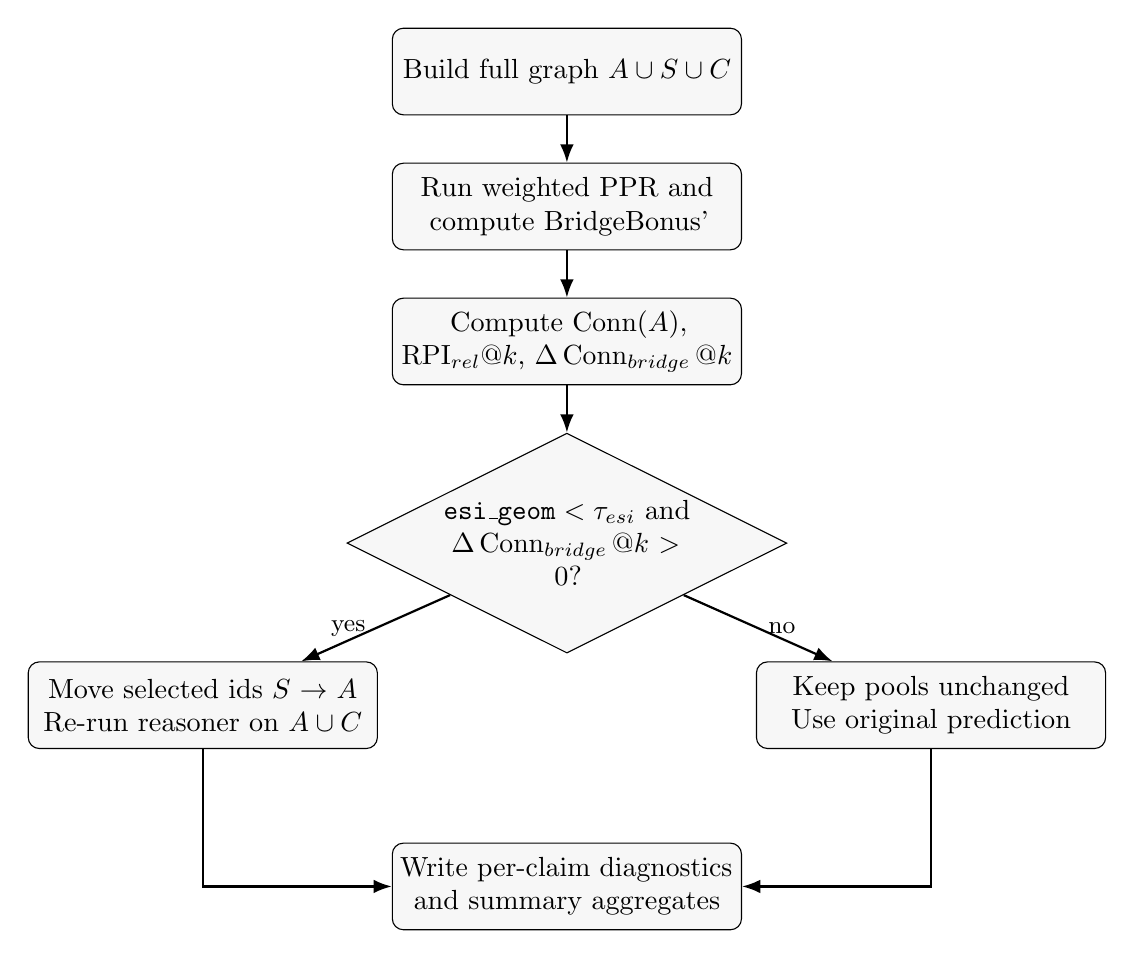
\begin{tikzpicture}[
  node distance=6mm and 8mm,
  block/.style={draw,rounded corners,align=center,text width=4.2cm,minimum height=1.1cm,fill=gray!6},
  decision/.style={draw,diamond,aspect=2,align=center,inner sep=1pt,text width=3.2cm,fill=gray!6},
  arrow/.style={-Latex,thick}
]
\node[block] (full) {Build full graph $A\cup S\cup C$};
\node[block, below=of full] (ppr) {Run weighted PPR and compute BridgeBonus'};
\node[block, below=of ppr] (eval) {Compute $\Conn(A)$, $\text{RPI}_{rel}@k$, $\Delta\Conn_{bridge}@k$};
\node[decision, below=of eval] (gate) {$\texttt{esi\_geom}<\tau_{esi}$ and $\Delta\Conn_{bridge}@k>0$?};
\node[block, below left=8mm and 10mm of gate] (yes) {Move selected ids $S\rightarrow A$\\Re-run reasoner on $A\cup C$};
\node[block, below right=8mm and 10mm of gate] (no) {Keep pools unchanged\\Use original prediction};
\node[block, below=of gate,yshift=-18mm] (log) {Write per-claim diagnostics and summary aggregates};

\draw[arrow] (full) -- (ppr);
\draw[arrow] (ppr) -- (eval);
\draw[arrow] (eval) -- (gate);
\draw[arrow] (gate) -- node[left,font=\small]{yes} (yes);
\draw[arrow] (gate) -- node[right,font=\small]{no} (no);
\draw[arrow] (yes) |- (log);
\draw[arrow] (no) |- (log);
\end{tikzpicture}
\end{adjustbox}
\caption{Recovery control flow with explicit trigger gate.}
\label{fig:recovery-flow}
\end{figure}

\subsection{Important edge-case semantics}
\begin{itemize}
\item If an anchor is not present in Active graph nodes, anchor-pair connectivity treats that pair as disconnected.
\item During bridge ranking, an $S$ edge connecting an Active component to an unseen node is treated as component-connecting.
\item These guards prevent false ``already connected'' interpretations in sparse graphs.
\end{itemize}


\section{Selective Prediction and Rationale Faithfulness}
\label{sec:selective-salience}

\subsection{Selective prediction objective}
FactKG labels are binary (SUPPORTED/REFUTED), but practical deployment requires controlled abstention when evidence sufficiency is low.
M3 computes an abstain score per claim and supports both:
\begin{itemize}
\item threshold-free risk-coverage behavior (\AURC{}),
\item optional fixed operating point via \texttt{tau\_abstain}.
\end{itemize}
This follows the selective classification framing where a model may abstain to improve reliability at chosen coverage levels \cite{geifman2017selective}.

\subsection{Abstain score used in code}
For class probabilities $\hat{\mathbf{p}}$ and sufficiency score $\texttt{esi\_geom}$:
\[
\texttt{abstain\_score}
= \alpha\cdot (1-\max(\hat{\mathbf{p}})) + (1-\alpha)\cdot (1-\texttt{esi\_geom}),
\]
with default $\alpha=0.5$.

\subsection{Risk-coverage evaluation and \AURC}
Given abstain scores and correctness labels:
\begin{enumerate}
\item sort claims by ascending abstain score (most answerable first),
\item reveal predictions progressively,
\item at each coverage level compute risk $=$ error rate among answered claims.
\end{enumerate}
Area under risk-coverage curve is computed by trapezoidal integration:
\[
\AURC = \sum_i (\phi_i-\phi_{i-1})\cdot\frac{R_i+R_{i-1}}{2}.
\]
Lower \AURC{} is better.

\subsection{Fixed operating point (\texttt{tau\_abstain})}
When \texttt{tau\_abstain} is set, claims with
\[
\texttt{abstain\_score} \le \texttt{tau\_abstain}
\]
are answered, and the rest are abstained.
Logged metrics:
\begin{itemize}
\item \texttt{coverage} $=$ answered / total,
\item \texttt{risk} $=$ errors among answered / answered,
\item \texttt{accuracy\_on\_answered},
\item \texttt{abstain\_rate} $=1-\texttt{coverage}$.
\end{itemize}

\subsection{Rationale edge extraction}
\texttt{extract\_top\_rationale\_edges} ranks edges by:
\[
\text{salience}_{\text{attn-pv}}(e)=\texttt{attention\_used}(e)\cdot \Rel(e).
\]
where \texttt{attention\_used} is class-conditioned:
\begin{itemize}
\item predicted class SUPPORTED: use \texttt{attention\_sup},
\item predicted class REFUTED: use \texttt{attention\_ref},
\item if no target class is passed: use $\max(\texttt{attention\_sup},\texttt{attention\_ref})$.
\end{itemize}
Default rationale budget: \texttt{rationale\_top\_n = 10}.

\subsection{Faithfulness checks implemented}
Two complementary checks are available:
\begin{enumerate}
\item \textbf{Leave-one-out (LOO):} remove one rationale edge at a time and measure confidence drop for predicted class.
\item \textbf{Grouped removal:} remove top-$k$ rationale edges together and measure confidence drop.
\end{enumerate}

Current boolean criterion is positive confidence drop:
\[
\texttt{is\_faithful} = [\Delta\text{confidence} > 0].
\]
M3 runs faithfulness only on the first \texttt{faithfulness\_subset\_size} claims (default $3$) to keep runtime bounded.

\subsection{What M3 logs for interpretability}
Per claim, M3 logs:
\begin{itemize}
\item \texttt{top\_rationale\_edges} with attention, PV relevance, and combined score,
\item \texttt{faithfulness\_loo} with per-edge confidence drops,
\item \texttt{salience\_results} (group removal) with aggregate drop.
\end{itemize}
Run-level summary adds counts such as:
\texttt{num\_faithful\_claims} and \texttt{num\_salience\_checked}.

\section{Worked Examples (Concept + Implementation Numbers)}
\label{sec:examples}

\subsection{Example A: Conceptual claim-level reasoning chain}
Claim:
\begin{quote}
\textit{``Barack Obama was born in Hawaii.''}
\end{quote}
Candidate triples might include:
\begin{itemize}
\item \texttt{(Barack\_Obama, birthPlace, Honolulu)}
\item \texttt{(Honolulu, isPartOf, Hawaii)}
\item \texttt{(Barack\_Obama, birthPlace, Kenya)}
\item \texttt{(Barack\_Obama, spouse, Michelle\_Obama)}
\end{itemize}

Interpretation under Component 2:
\begin{itemize}
\item support stream increases flow along entailment-leaning edges,
\item refute stream preserves contradiction edge to Kenya,
\item neutral spouse edge receives low bridge value after neutrality cap.
\end{itemize}
This example illustrates why dual streams and bridge capping are both necessary.

\subsection{Example B: M2 policy-aware recovery numbers (from run logs)}
This is the exact synthetic M2 pattern used in dev notes:
anchors: $A, C$.

Active edges:
\begin{itemize}
\item \texttt{a1}: $A\leftrightarrow B$ with $(p_{ent},p_{con},p_{neu})=(0.65,0.05,0.30)$
\item \texttt{a2}: $C\leftrightarrow D$ with $(0.62,0.06,0.32)$
\end{itemize}

Suspended edges include one true bridge:
\texttt{s\_bridge: B\leftrightarrow C} with $(0.52,0.08,0.12)$,
and three high-rel but noisy non-bridges.

Mask values:
\begin{align}
 m_{sup}(\texttt{s\_bad1}) &= \sigmoid(4\cdot0.83-2)=0.789182, \\
 m_{ref}(\texttt{s\_bad1}) &= \sigmoid(4\cdot0.05-2)=0.141851, \\
 m_{sup}(\texttt{s\_bridge}) &= \sigmoid(4\cdot0.52-2)=0.519989.
\end{align}

Bridge scores from recorded run:
\begin{align}
\text{BridgeBonus}'(\texttt{s\_bridge}) &= 0.0189136, \\
\text{BridgeBonus}'(\texttt{s\_bad1}) &= 0.0103967, \\
\text{BridgeBonus}'(\texttt{s\_bad2}) &= 0.0099324, \\
\text{BridgeBonus}'(\texttt{s\_bad3}) &= 0.0046006.
\end{align}

Connectivity outcomes at $k=3$:
\begin{itemize}
\item $\Conn(A)=0.0$ (anchors disconnected),
\item rel-policy top-3 keeps anchors disconnected: $\text{RPI}_{rel}@3=0.0$,
\item bridge-policy top-3 includes \texttt{s\_bridge}: $\Delta\Conn_{bridge}@3=1.0$.
\end{itemize}
With \texttt{esi\_geom}=0.2 and $\tau_{esi}=0.3$, recovery triggers and reruns with moved edges.

\subsection{Example C: M3 abstention and salience numbers}
For synthetic claim \texttt{synthetic\_m3\_0}, recorded post-recovery probabilities were:
\[
P(\text{SUPPORTED})=0.3444325990,\quad P(\text{REFUTED})=0.6555674010.
\]
Thus confidence is $0.6555674010$.
With \texttt{esi\_geom}=0.2 and $\alpha=0.5$:
\begin{align}
\texttt{abstain\_score}
&=0.5(1-0.6555674010)+0.5(1-0.2) \\
&=0.5722162995.
\end{align}

Top rationale edge example:
\begin{align}
\texttt{attention\_max} &= 0.6899744811, \\
\Rel(e) &= 0.75, \\
\text{salience}_{attn-pv} &= 0.6899744811\cdot0.75=0.5174808608.
\end{align}

Leave-one-out faithfulness sample:
removing one top edge changed confidence from $0.6555674010$ to $0.6379624966$,
a drop of $0.0176049045$.


\section{Code Mapping, Runtime Commands, and Locked Defaults}
\label{sec:code-mapping}

\subsection{Module-to-responsibility map}
\begin{table}[H]
\centering
\begin{tabular}{@{}p{0.34\linewidth}p{0.58\linewidth}@{}}
\toprule
Module & Responsibility \\
\midrule
\texttt{src/component2/types.py} & Input normalization, schema validation, label mapping. \\
\texttt{src/component2/anchor\_adapter\_factkg.py} & Inject FactKG \texttt{Entity\_set} anchors by \texttt{claim\_id}/\texttt{claim\_text}; emits load-issue warnings and exposes load diagnostics. \\
\texttt{src/component2/anchor\_selector.py} & Seed-first anchor selection with text and degree fallbacks. \\
\texttt{src/component2/graph\_builder.py} & Build \texttt{EvidenceGraph} from selected pools and triples. \\
\texttt{src/component2/reasoner.py} & Masked dual-stream relation-aware graph reasoner and salience output. \\
\texttt{src/component2/bridge\_rescue.py} & Weighted PPR node scoring and bridge bonus computation. \\
\texttt{src/component2/recovery.py} & Policy-aware recovery metrics, trigger gate, and S$\rightarrow$A move. \\
\texttt{src/component2/selective.py} & Abstain score, risk-coverage points, and \AURC{} calculation. \\
\texttt{src/component2/salience.py} & Top rationale extraction and faithfulness diagnostics. \\
\texttt{src/component2/run\_m1.py} & M1 smoke runner. \\
\texttt{src/component2/run\_m2.py} & M2 smoke runner with recovery diagnostics. \\
\texttt{src/component2/run\_m3.py} & M3 smoke runner with selective prediction and rationale checks. \\
\bottomrule
\end{tabular}
\caption{Direct code map for implementation traceability.}
\label{tab:module-map}
\end{table}

\subsection{Default configuration values (\texttt{Component2Config})}
The table below mirrors \texttt{src/component2/config.py} exactly.

\begin{longtable}{@{}p{0.35\linewidth}p{0.18\linewidth}p{0.40\linewidth}@{}}
\toprule
Key & Default & Used for \\
\midrule
\endfirsthead
\toprule
Key & Default & Used for \\
\midrule
\endhead
\texttt{anchor\_max\_k} & 5 & Maximum anchors selected per claim. \\
\texttt{anchor\_fallback\_degree\_k} & 2 & Degree fallback candidates for anchors. \\
\texttt{factkg\_data\_dir} & data/factkg & Base folder for FactKG anchor pickles. \\
\texttt{factkg\_train\_pickle} & factkg\_train.pickle & Train split anchor source. \\
\texttt{factkg\_val\_pickle} & factkg\_dev.pickle & Dev/val split anchor source. \\
\texttt{factkg\_test\_pickle} & factkg\_test.pickle & Test split anchor source. \\
\texttt{hidden\_dim} & 256 & Node hidden dimension in reasoner. \\
\texttt{num\_heads} & 4 & Attention heads in reasoner. \\
\texttt{rel\_emb\_dim} & 64 & Relation embedding dimension. \\
\texttt{random\_seed} & 13 & Deterministic initialization and hashing. \\
\texttt{message\_passing\_layers} & 1 & Stream update depth. \\
\texttt{mask\_sup\_scale} & 4.0 & Support mask coefficient. \\
\texttt{mask\_sup\_bias} & -2.0 & Support mask bias. \\
\texttt{mask\_ref\_scale} & 4.0 & Refute mask coefficient. \\
\texttt{mask\_ref\_bias} & -2.0 & Refute mask bias. \\
\texttt{ppr\_epsilon} & 0.001 & Edge weight floor for diffusion. \\
\texttt{neutral\_cap\_gamma} & 2.0 & Neutrality penalty exponent in bridge score. \\
\texttt{ppr\_alpha} & 0.15 & Restart mixing factor in PPR iteration. \\
\texttt{ppr\_max\_iters} & 100 & Maximum PPR iterations. \\
\texttt{ppr\_tolerance} & 1e-6 & PPR convergence threshold ($L_1$ residual). \\
\texttt{recovery\_tau\_esi} & 0.3 & Insufficiency threshold for recovery gate. \\
\texttt{recovery\_tau\_rpi\_legacy} & 0.15 & Legacy reference only (not trigger gate). \\
\texttt{recovery\_top\_k} & 3 & Number of Suspended edges considered for move. \\
\texttt{abstain\_alpha} & 0.5 & Confidence-vs-sufficiency blend in abstain score. \\
\texttt{tau\_abstain} & None & Optional fixed abstention operating point. \\
\texttt{compute\_risk\_coverage\_sweep} & True & Enable risk-coverage curve and \AURC{}. \\
\texttt{rationale\_top\_n} & 10 & Number of rationale edges returned. \\
\texttt{faithfulness\_subset\_size} & 3 & Number of claims for expensive faithfulness checks. \\
\texttt{faithfulness\_top\_k\_edges} & 10 & Maximum rationale edges removed in checks. \\
\texttt{smoke\_max\_claims} & 5 & Default smoke-run batch size. \\
\texttt{numpy\_edge\_warn\_threshold} & 5000 & Emit numpy-mode performance warning above this edge count. \\
\bottomrule
\end{longtable}

\subsection{Recommended run commands}
\begin{verbatim}
# M1
PYTHONPATH=src python3 -m component2.run_m1 --max-claims 5 --output-root logs/component2

# M2
PYTHONPATH=src python3 -m component2.run_m2 --max-claims 5 --output-root logs/component2

# M3 (Component 1 logs mode by default path)
PYTHONPATH=src python3 -m component2.run_m3 --max-claims 5 --output-root logs/component2

# M3 with fixed abstention operating point only (disable sweep)
PYTHONPATH=src python3 -m component2.run_m3 --max-claims 5 --tau-abstain 0.55 --no-risk-coverage-sweep
\end{verbatim}

\subsection{Run-level summary metrics to monitor}
\begin{itemize}
\item M1: \texttt{loss}, \texttt{relation\_vocab\_size}.
\item M2: \texttt{num\_recovered}, \texttt{avg\_delta\_conn\_bridge\_at\_k}, \texttt{num\_ppr\_not\_converged}.
\item M3: \texttt{aurc} (if sweep enabled), fixed-point selective metrics at \texttt{tau\_abstain} (if set), \texttt{num\_faithful\_claims}, \texttt{num\_salience\_checked}, plus PPR diagnostics counters.
\item All runners: \texttt{anchor\_source\_counts}, \texttt{claims\_missing\_pickle\_mapping}, and numpy perf warning counters.
\item Runtime logs: watch for \texttt{FactKGAnchorAdapter} load warnings indicating missing/invalid anchor pickles or zero extracted mappings.
\end{itemize}

\section{Glossary and Explainer Checklist}
\label{sec:glossary}

\subsection{Glossary}
\begin{table}[H]
\centering
\begin{tabular}{@{}p{0.24\linewidth}p{0.68\linewidth}@{}}
\toprule
Term & Definition \\
\midrule
PV & Premise Validation probability distribution over entail/contradict/neutral. \\
Active ($A$) & Evidence currently used by the reasoner. \\
Suspended ($S$) & Evidence held out unless recovery trigger opens it. \\
Counter ($C$) & Contradiction-oriented evidence retained for refutation signal. \\
Dual-stream & Two separate message-passing streams: support and refute. \\
Bridge rescue & Diffusion-based scoring to detect structurally useful edges. \\
Recovery & One-step move of selected edges from $S$ to $A$ under trigger gate. \\
Selective prediction & Ability to abstain based on uncertainty + insufficiency. \\
\AURC{} & Area under risk-coverage curve; lower is better. \\
Rationale faithfulness & Whether removing important edges reduces predicted-class confidence. \\
\bottomrule
\end{tabular}
\caption{Quick definitions for presentation and review settings.}
\end{table}

\subsection{Checklist for explaining Component 2 to others}
Use this sequence for clean technical explanation:
\begin{enumerate}
\item Start with the interface contract: claim row, triple row, and required probability constraints.
\item Explain why $A/S/C$ pools are separated and why Component 2 reasons on $A\cup C$ but scores bridges on $A\cup S\cup C$.
\item Show PV masks and dual-stream attention to clarify how support/refute signals are preserved.
\item Explain recovery gate: low \texttt{esi\_geom} is necessary but not sufficient; predicted bridge connectivity gain must be positive.
\item Present selective prediction and \AURC{} to show reliability beyond top-1 accuracy.
\item End with rationale faithfulness to show interpretability is tested, not only visualized.
\end{enumerate}

\subsection{Current limitations (for transparent academic reporting)}
\begin{itemize}
\item The reasoner is currently a deterministic NumPy implementation, not a trained deep model checkpoint.
\item Recovery is one-step and greedy top-$k$; no multi-round optimization is implemented.
\item Faithfulness criterion uses confidence-drop positivity; stronger causal tests can be added later.
\item M3 behavior depends on quality/completeness of Component 1 pair logs in compatibility mode.
\end{itemize}



\bibliographystyle{plain}
\bibliography{component2_refs}

\end{document}
